% Revised ACL 2027 submission: main body (Sections 1-8, Limitations, Ethics).
% The original Appendices A-Q are unchanged except for the edits listed in
% ../修改对照表.md; the new Appendices R-X are in appendix_new.tex.
\documentclass[11pt]{article}
\usepackage[review]{acl}
\usepackage{times}
\usepackage{latexsym}
\usepackage[T1]{fontenc}
\usepackage[utf8]{inputenc}
\usepackage{microtype}
%\usepackage{inconsolata}
\usepackage{graphicx}
\usepackage{amsmath,amssymb,amsthm}
\usepackage{booktabs}
\usepackage{algorithm}
\usepackage[noend]{algpseudocode}

\newtheorem{theorem}{Theorem}
\newtheorem{proposition}{Proposition}
\newtheorem{corollary}{Corollary}
\newtheorem{lemma}{Lemma}

\newcommand{\Qj}{Q_{\mathrm{joint}}}
\newcommand{\Qu}{Q_{\cup,\mathrm{sep}}}
\newcommand{\Qs}{Q_{\mathrm{split}}}
\newcommand{\Qx}{Q_{\mathrm{exact}}}
\newcommand{\bH}{b_H}
\newcommand{\Sz}{S_0}
\newcommand{\ind}{\mathbf{1}}
\newcommand{\app}[1]{Appendix~#1}

\title{How Many Evaluator Scores Certify Output Retention\\ Under a Churn Budget?}
\author{Anonymous ACL submission}

\begin{document}
\maketitle

\begin{abstract}
Replacing an evaluator can change which language outputs pass an ensemble cutoff. We study the score evidence needed to certify that a returned subset meets an average normalized churn budget and retains a count within a specified tolerance of the full-information optimum under that budget. The normalization, cutoff and a finite family of single-evaluator replacements are fixed, and the guarantees hold for every score completion consistent with the observed entries. We characterize minimum certificates chosen with full-score knowledge and verified from revealed entries only. For odd median pools, the evidence for feasibility and the evidence excluding larger retained sets are disjoint, which yields closed-form minima. Mean and even-median pools allow one observation to serve both purposes. Under exact count certification from an empty history, we construct mean-pooling families whose joint certificate approaches half the size of the best union of separately minimum certificates. Across 1,920 mean targets from cached RewardBench~2 and five WMT panels, numerical optimization finds modest joint gains in 89 targets, all of which require exclusion evidence, and the corresponding whole-column targets show no gain. Discovering a two-entry certificate can require queries linear in batch size, even with positive count tolerance. We also extend the analysis to weighted and per-replacement churn objectives and to verifiable cross-entry score constraints. Certificate size, discovery cost and inference time require separate evaluation, and retention stability does not certify output quality.
\end{abstract}

\section{Introduction}
Reward models, translation metrics and LLM judges score language outputs \citep{malik2026rewardbench2,freitag2023wmt23,zheng2023judging}, and ensembles of such evaluators are often used to filter a batch \citep{coste2024ensembles,eisenstein2024herding}. Evaluators are replaced over time. Before rescoring a selected batch after replacing one ensemble member, an analyst may want evidence that many outputs would keep their selection status within a declared churn allowance. Returning nothing is always feasible, so a useful certificate must also bound how many outputs are lost relative to the best budget-feasible retention.

We study this problem for a fixed batch. A base pool of evaluators selects outputs whose median or mean normalized score reaches a cutoff, and a finite family of candidate evaluators defines every single-member replacement. Candidate scores on the batch are initially unknown and can be revealed entry by entry. A \emph{certificate} is a set of revealed entries from which a verifier can conclude, for every completion of the unrevealed scores, that a returned subset meets the churn budget and that its count is within $\varepsilon$ outputs of the optimum. This guarantee is deterministic and completion-wise. It complements conformal and selective risk control, which bound expected risk under exchangeability \citep{angelopoulos2024crc,bai2026score}.

Our contributions are as follows.
(i) We define safety evidence, which certifies feasibility, and exclusion evidence, which rules out larger retained sets, and we show that both bounds are sharp under the declared completion model (Section~\ref{sec:cert}).
(ii) For odd medians the two kinds of evidence are disjoint, giving closed-form minimum certificates. For mean and even-median pools a single entry can serve both, and we give an exact joint program together with a tight factor-two separation from the best union of separately minimum witnesses (Section~\ref{sec:minimum}).
(iii) We separate certificate size from discovery: two-entry certificates can require queries linear in batch size even at positive tolerance (Section~\ref{sec:acquire}).
(iv) On RewardBench~2, WMT and SummEval panels we measure inspection, minimum evidence, and joint gains, and we identify when sharing evidence helps (Section~\ref{sec:exp}).
(v) We extend the theory to weighted and per-replacement churn objectives and to verifiable cross-entry constraints (Appendices~R--S).
Stability differs from quality: evaluator agreement can coexist with shared errors and reward hacking \citep{eisenstein2024herding}.

\section{Related Work}
\paragraph{Risk control and judge stability.} Conformal risk control (CRC) bounds an expected monotone loss \citep{angelopoulos2024crc,yeh2025crt}, and risk-controlling prediction sets give high-probability bounds \citep{bates2021rcps}. SCoRE, SCOPE and multi-expert CRC address selective risk, pairwise acceptance and multiple judges \citep{bai2026score,badshah2026scope,cheng2026multiexpert}. Replicable calibration stabilizes thresholds across samples \citep{papamichalis2026replicable}. LLM judges are sensitive to position and prompt variations \citep{wang2024fair,thakur2024judges}, and ensemble agreement need not exclude common errors \citep{afrin2026ensembles}. Predictive churn has been studied for model updates and training-sample changes \citep{milanifard2016churn,watsondaniels2025churn,prastalo2026churn}, and fixed-threshold routing can change even with matching class predictions \citep{kim2026lottery}. Our guarantee instead concerns one fixed batch, holds for every consistent score completion, and is stated relative to a declared replacement family.

\paragraph{Verification, discovery and robust selection.} Priced information and matroid verification distinguish proof size from discovery cost \citep{charikar2002priced,diwan2026matroid}, and Boolean evaluation studies adaptive queries \citep{deshpande2016submodular,gkenosis2018scoreclassification}. Robust selection and knapsack problems choose queries before uncertain parameters are resolved \citep{chen2026robustselection,goerigk2015knapsack}, often with budgeted uncertainty sets \citep{bertsimas2004price}; uncertain-profit knapsack certifies good packings and excludes better ones under resource augmentation \citep{schloter2025knapsack}. Recoverable selection permits later exchanges \citep{chassein2018recoverable}, and covering and query-competitive models study sharing and discovery \citep{megow2023covering,erlebach2015querycompetitive,erlebach2021parallel}. These models leave costs or profits uncertain. Here the uncertainty is a matrix of candidate scores under a known pooling rule, and we verify feasibility and optimality for a fixed scenario family rather than solve a min--max design problem. Unlike black-box certification \citep{blanc2022certification,gupta2023monotone}, we query a fixed matrix.

\paragraph{Top-$k$ with partial information.} Sorted-list aggregation supports sorted and random accesses \citep{fagin2003middleware}; our certificates assume no sorted oracle. Top-$k$ queries over uncertain or incomplete data compute possible and certain answers \citep{imielinski1984incomplete,soliman2007uncertaintopk,amarilli2017topk}, and partial voting profiles admit necessary and possible winners \citep{imber2020topk}. Our safe and optimistic counts play the role of certain and possible retention, but the object certified is a budget-constrained optimum over a replacement family, which leads to different certificate combinatorics. Ranking robustness covers weight changes and word attacks \citep{asudeh2018stable,wu2022wordsub}; PAC selection, Col-Bandit and budget-adaptive ranking acquire scores adaptively \citep{kalyanakrishnan2012pac,pony2026colbandit,oettershagen2026topk}. Selective ensembles, pruning and early exit reduce scoring cost \citep{black2022selective,li2022pruning,inoue2019adaptive,busolin2021earlyexit}, and Best-of-Evidence queries factors within a fixed pool \citep{zhang2026bestofevidence}. MT filtering and metric biases motivate separate quality assessment \citep{perrella2024beyond,shayegh2025adequacy}.

\section{Selection under Evaluator Replacements}
\label{sec:setup}
Rows index outputs and columns index evaluators. Pools $P$ and $R$ contain $M\ge1$ base and $T\ge1$ candidate evaluators. Normalization maps and a cutoff $0<t_0\le1$ are fitted on a reference split of scored outputs (here, \emph{reference} denotes the fitting split, not a human reference translation). Write $s_e(i)\in[0,1]$ for normalized scores. Replacing base member $j$ by candidate $r$ gives the pool $P^{j\to r}$; the $H=MT$ replacements have uniform weight. The maps and cutoff remain fixed. Base scores are visible; queries reveal candidate test scores.

The base list is $\Sz(P)=\{i: c_P(i)\ge t_0\}$, where $c_P$ is median or mean consensus; an even-sized median averages the two central scores, and cutoff ties are included. For a batch of $N$ outputs, fix a nominal selection fraction $q\in(0,1]$ and the nominal count $k=\max(1,\mathrm{round}(qN))$ (half-integers round to even). The count $k$ scales the risk and imposes no return quota. With $\sigma_Q(i)=\ind[i\in\Sz(Q)]$, base scores and one candidate score determine all $M$ replacement outcomes of a row. Define the flip count and row total
\begin{equation}
f_{ir}=\sum_{j=1}^{M}\ind[\sigma_P(i)\neq\sigma_{P^{j\to r}}(i)],\quad F_i=\sum_{r=1}^{T}f_{ir}.
\label{eq:flips}
\end{equation}
A commitment mask $C$ fixes baseline decisions without review and returns $\Sz(P)\cap C$. Its average normalized churn over the declared replacements is
\begin{equation}
\begin{split}
R(C)&=\frac1H\sum_{j,r}\frac{|(\Sz(P)\triangle \Sz(P^{j\to r}))\cap C|}{2k}\\
&=\frac{\sum_{i\in C}F_i}{2kH}.
\end{split}
\label{eq:risk}
\end{equation}
Decisions outside $C$ are referred for review. We maximize the returned count subject to $R(C)\le\alpha$. Nonselected outputs do not increase the returned count and receive no dedicated entry queries, and an exclusion is committed only when base scores rule out every membership flip. With all costs observed, the integer flip budget is $\bH=\lfloor 2k\alpha H\rfloor$; sorting selected outputs by increasing $F_i$ and taking the longest prefix within $\bH$ gives the full-information optimum $V^*$.

\begin{table}[t]
\centering\footnotesize
\setlength{\tabcolsep}{2pt}
\begin{tabular}{@{}lll@{}}
\toprule
Quantity & Definition & Example\\
\midrule
Churn budget & $R(C)\le\alpha$, Eq.~\eqref{eq:risk} & $.10$\\
Changes/replacement & $\rho=2k\alpha$ & $0.4$\\
Flip budget & $\bH=\lfloor\rho H\rfloor$ & $8$\\
Oppositions (odd $M$) & $b=\lfloor \bH/(h+1)\rfloor$ & $2$\\
Count tolerance & $V^+-V^-\le\varepsilon$ & $\varepsilon\ge0$\\
Active inspection & $100\,Q/(mT)$ & --\\
\bottomrule
\end{tabular}
\caption{Units and conversions. The example uses $M=7$ ($h=3$), $T=3$ and $k=2$, so $H=21$ (Appendix A.7). Because $2k$ is a fixed nominal scale, $R(C)>1$ is possible when many outputs are returned; only $2k\alpha$ matters for feasibility (Appendix L).}
\label{tab:units}
\end{table}

\paragraph{Units.} Table~\ref{tab:units} collects the conversions. Allowing $\rho$ average membership changes per replacement gives $\alpha=\rho/(2k)$. This is an average replacement allowance, not a per-replacement limit or a review-capacity quota.

\paragraph{Choice of risk objective.} The uniform average in Eq.~\eqref{eq:risk} makes the full-information problem a sorted prefix and yields the closed forms below. Three alternatives are natural. \emph{Fixed nonnegative replacement weights} preserve every bound and the sorted-prefix argument; Theorem~\ref{thm:joint} extends with column-dependent caps, and odd-median evidence remains disjoint (Appendix~R.1). \emph{Certifying each single replacement}, i.e., a per-replacement cap $\max_{j,r}|\cdot|/(2k)\le\alpha$, keeps verification of a given mask linear-time and sharp, but computing the optimal retained count becomes NP-hard even with full information, so count gaps require integer programs (Appendix~R.2). This matters in practice: 6,985 of 15,360 average-certified masks exceed $.10$ for at least one individual replacement (Appendix I). \emph{A known single replacement} reduces to one candidate column with Boolean row costs. Uniform weights correspond to a replacement chosen uniformly from the declared family.

\section{Certificates from Partial Scores}
\label{sec:cert}
A certificate uses visible base scores and queried candidate scores to verify churn feasibility and bound the count shortfall. One entry query determines all $M$ replacement outcomes of its row. Let $f_i(x)$ count flips when a candidate assigns score $x$ to output $i$, so $f_{ir}=f_i(s_r(i))$ and $p_i=\max_{x\in[0,1]}f_i(x)$. Under either pooling rule, replacement consensus is nondecreasing in $x$; for selected outputs $f_i$ is nonincreasing, with maximum $p_i$ at $x=0$ and zero at $x=1$. Visible base scores determine $p_i$. After $t_i$ queries on row $i$, let $\ell_i$ sum their observed contributions. Bounding each unobserved count between zero and $p_i$ gives
\begin{equation}
\ell_i\le F_i\le u_i=\ell_i+(T-t_i)p_i.
\label{eq:bounds}
\end{equation}
For nonnegative costs $w$, define the retention capacity $V(w)=\max\{|C\cap\Sz(P)|:\sum_{i\in C}w_i\le\bH\}$, computed by sorting. Maximizing retention under $u$ yields a mask returning $V^-=V(u)$ outputs that is feasible for every consistent completion; the optimistic count $V^+=V(\ell)$ is attained in some completion.

\paragraph{The completion model.} Unobserved scores range freely over $[0,1]$. This is a set of possible matrices, not a statistical assumption: assigning every unobserved entry its zero-flip endpoint realizes $\ell$, and assigning its maximum-flip endpoint realizes $u$. We use this worst-case set because correlations among evaluators, however strong on reference data, do not by themselves guarantee where an unseen test score lies; predictions therefore guide query order but never tighten bounds. Valid cross-entry constraints can only shrink the completion set: every certificate in this paper remains valid under them and minimum certificates can only become smaller. A verifiable class stays tractable. If the constrained completion set is a lattice, with coordinatewise greatest and least elements, then the same two completions give sharp bounds. This covers per-entry score supports, monotonicity constraints and Lipschitz-with-slack constraints across outputs for each evaluator, whose envelopes are computed in linear time per query (Propositions~18--19, Appendix~S). In a controlled study with valid Lipschitz-with-slack constraints, primary-stop inspection falls from 72--96\% to 4--68\% of active entries, depending on the slack and depth; a misspecified constant produced invalid certificates in 12 of 80 exact-stop runs, so such constraints must be justified externally.

\begin{proposition}[Safe retention and stopping]
\label{prop:safe}
At any adaptive query history, let $C^-$ maximize retained count subject to the upper-cost budget. Then $R(C^-)\le\alpha$ and $V^-\le V^*\le V^+$. If $V^+-V^-\le\varepsilon$, its returned count is at most $\varepsilon$ outputs below $V^*$. Under the declared replacement family and completion model, these guarantees hold for every acquisition order and stopping time.
\end{proposition}
\begin{proof}
Equation~\eqref{eq:bounds} bounds each true cost. Upper-cost feasibility implies true feasibility, which implies lower-cost feasibility; maximizing cardinality gives the count bounds. The returned count is $V^-$, so its shortfall is at most the gap.
\end{proof}
Integer $\varepsilon\ge0$ bounds count shortfall, and zero requires count optimality. Full revelation gives $V^-=V^+=V^*$. An output is structurally invariant ($p_i=0$) if no candidate score can change its membership; noninvariant outputs can still have zero true cost. Zero-query retention uses upper costs $Tp_i$ and can admit noninvariant outputs within budget. Let $m_0=|\{i\in\Sz:p_i=0\}|$ count invariant selected rows; only the $m=|\{i\in\Sz:p_i>0\}|$ active selected rows are eligible for entry queries, and active inspection is $Q/(mT)$ for $Q$ entry queries (zero when $m=0$). The safe count cannot decrease, although retained sets need not be nested.

\section{Minimum Certificate Complexity}
\label{sec:minimum}
\paragraph{Odd medians: disjoint evidence.} For $M=2h+1$, median selection requires $h+1$ votes at or above $t_0$, and a single replacement changes at most one vote. Selected rows with at least $h+2$ votes are invariant; those with exactly $h+1$ form the boundary set $B$, and a below-cutoff candidate excludes a boundary row exactly when it replaces one of its $h+1$ voting members. Thus $p_i=h+1$ on $B$. For $i\in B$ define opposition bits $y_{ir}=\ind[s_r(i)<t_0]$ and row sums $z_i=\sum_r y_{ir}$, so $F_i=(h+1)z_i$. In opposition units, feasibility is exactly $\sum_{i\in C\cap B}z_i\le b$ with $b=\lfloor \bH/(h+1)\rfloor$ (Table~\ref{tab:units}). On a boundary row, an \emph{agreement} (candidate score at or above the cutoff) lowers the upper bound by one opposition, and an \emph{opposition} raises the lower bound by one: with $a_i$ agreements and $o_i$ oppositions observed, $o_i\le z_i\le T-a_i$. An offline constructor uses the true bit matrix to choose entries; the verifier sees only revealed entries and checks every consistent Boolean completion.

\begin{theorem}[Safety witness]
\label{thm:safety}
If the true matrix admits a feasible set of $L$ boundary rows, the minimum number of observations certifying that an $L$-row set is feasible under every consistent completion is $Q_{\mathrm{safe}}(L)=\max\{0,LT-b\}$. If no $L$-row set is truly feasible, no certificate exists.
\end{theorem}
An $L$-row set starts with upper cost $LT$, and only agreements reduce it, one unit each; any truly feasible set contains enough agreements (Appendix A gives proofs and a worked example). Feasibility need not establish optimality. Let $z_{(1)}\le\dots\le z_{(m)}$ and let $L$ be the largest prefix size with sum at most $b$; the full retained optimum is $m_0+L$.

\begin{theorem}[Exact optimality witness]
\label{thm:exact}
If $L=m$, the minimum certificate proving exact optimality is $\max(0,mT-b)$. Otherwise set $p=L+1$, $B_0=b+1$, $D(t)=\sum_{i=1}^{p}\min(z_{(i)},t)$ and $t^*=\min\{t\in\{0,\dots,T\}:D(t)\ge B_0\}$. The exact offline certificate size is
\begin{equation}
\Qx=\max(0,LT-b)+B_0+(m-p)t^*.
\label{eq:qexact}
\end{equation}
\end{theorem}
The exclusion part reveals $b+1$ oppositions across the $p$ cheapest rows, capped at $\min(z_{(i)},t^*)$, and $t^*$ oppositions in every remaining row. These cells are disjoint from the safety agreements, so the two costs add. With certified safe boundary count $s$, tolerance $\varepsilon$ requires every $(s+\varepsilon+1)$-row boundary set to be excluded unless that size exceeds $m$.

\begin{corollary}[Minimum gap witness]
\label{cor:gap}
Let $L^*$ be the true optimal boundary count and $\varepsilon\ge0$ an integer. For $L^*<p\le m$, let $D_p(t)=\sum_{i=1}^{p}\min(z_{(i)},t)$, $t_p=\min\{t:D_p(t)>b\}$ and $E(p)=b+1+(m-p)t_p$; for $p>m$ set $E(p)=0$. Then
\begin{equation}
Q_\varepsilon=\min_{s\in\mathcal S_\varepsilon}\big[\max(0,sT-b)+E(s+\varepsilon+1)\big],
\label{eq:qeps}
\end{equation}
with $\mathcal S_\varepsilon=\{\max(0,L^*-\varepsilon),\dots,L^*\}$. In particular $Q_0=\Qx$.
\end{corollary}
These minima lower-bound entry queries for the same instance, budget, model and tolerance from an empty history (Appendix A.6); residual witnesses account for existing observations (Appendix M.4).

\begin{figure}[t]
\centering
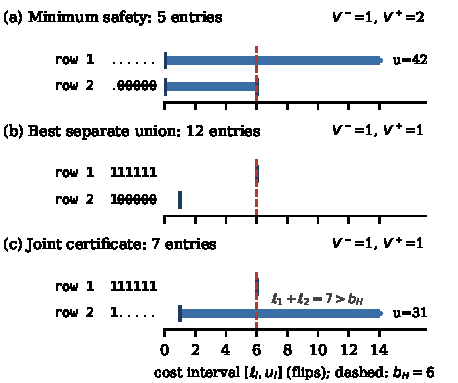
\includegraphics[width=\columnwidth]{figures/fig1_joint_example.pdf}
\caption{One mean-pooling entry can serve safety and exclusion (Proposition~9 at $T=6$; caps $p=(7,6)$, $\bH=6$, exact stopping). Digits are revealed flip counts; dots are unqueried. Bars show $[\ell_i,u_i]$. (a) The shortest safety proof certifies row~2. (b) Its best union with the unique minimum exclusion witness reveals all 12 entries. (c) Retaining row~1 instead uses the six entries that exclusion already needs: they set $u_1=6\le\bH$ (safety) and, with one entry of row~2, make the two smallest lower costs sum to $7\ge\bH+1$ (exclusion).}
\label{fig:joint}
\end{figure}

\paragraph{Joint evidence: mean and even medians.} An entry with true contribution $f_{ir}$ raises its row's lower cost by $f_{ir}$ and reduces its upper cost by $p_i-f_{ir}$. Mean pooling can have integer contributions $0<f_{ir}<p_i$, so one query contributes to both proofs. Figure~\ref{fig:joint} shows the mechanism. Exclusion of every $p$-row set is equivalent to the $p$ smallest lower costs summing to at least $\bH+1$, which we write with a single threshold $t$ as $\sum_i(t-\ell_i)_+\le pt-\bH-1$ (Lemma~1, Appendix M.5). In the figure, the six entries of row~1 are needed for exclusion; choosing row~1 as the retained row turns them into a safety proof as well, so the longer safety proof yields the shorter complete certificate.

For a history $\mathcal O$, let $\ell_i^0,u_i^0$ be its row bounds and $U_i$ its unqueried candidates. Using true contributions offline, define $\mathcal D_i=\{(|J|,\sum_{r\in J}f_{ir}):J\subseteq U_i\}$. A state $(a_i,v_i)$ gives $\ell_i=\ell_i^0+v_i$ and $u_i=u_i^0-a_ip_i+v_i$. Let $L^*$ be the true optimal active count.

\begin{theorem}[Joint entry witness]
\label{thm:joint}
For the fixed true matrix, history $\mathcal O$ and integer $\varepsilon\ge0$, the minimum additional entry count $\Qj$ is $\min\sum_ia_i$ over $s\in\{\max(0,L^*-\varepsilon),\dots,L^*\}$, row states in $\mathcal D_i$ and a safe set $C$ of $s$ active rows with $\sum_{i\in C}u_i\le\bH$. If $p=s+\varepsilon+1\le m$, also require an integer $0\le t\le TM$ such that $\sum_i(t-\ell_i)_+\le pt-\bH-1$, where $(x)_+=\max(0,x)$. For $p>m$, exclusion is automatic.
\end{theorem}
Every successful query set induces reachable row states and a safe count, and every feasible state choice is attained by a query set of the same size (Appendix M.5). The offline dynamic program is polynomial in explicit $m,T,M$ but has a budget-indexed grid; an equivalent integer program groups equal within-row outcomes into $G$ row--outcome groups with $O(G+m)$ variables and constraints per safe-count target, without guaranteeing polynomial solver time. On the 1,920 full mean targets, this program closes 1,876 within a nominal 60 seconds, and constructed-score grids up to $N=8192$, $T=65$ close in four of eight cases (Appendix M.7). Its optima are identical across HiGHS settings and CBC on our solver-sensitivity grid (Appendix~W).

\paragraph{What joint optimization adds.} Let $\Qs$ minimize the sum of separately minimum safety and exclusion sizes over admissible safe counts, and let $\Qu$ minimize the union of tied minimum safety and exclusion witnesses at the same count, then over counts. For the same instance, history and tolerance,
\begin{equation}
\Qj\le\Qu\le\Qs\le2\Qj.
\label{eq:sandwich}
\end{equation}
Realizable mean families attain $\Qu/\Qj\to2$, or $53/30$ at fixed $M=7$, $\alpha=.10$, with empty history and exact stopping (Appendix M.8). The sandwich holds for any fixed nonnegative replacement weights, and the factor-two family persists for every weight vector within relative distance $1/(2MT)$ of uniform (Proposition~14, Appendix~R.1).

\paragraph{When can sharing help?} Three conditions are checkable before any candidate-test score is seen. A strict gain $\Qu>\Qj$ requires (a) a nonzero initial gap, $|\Sz|-V^-(0)>\varepsilon$, and (b) an active row with two distinct replacement thresholds in $(0,1]$, since otherwise every contribution is $0$ or $p_i$ and Corollary~3 gives equality; odd medians never satisfy (b). Ex post, (c) a gain requires a witness that cannot certify exclusion automatically, and all 1,831 no-gain NLP targets have a witness with $V^-+\varepsilon\ge|\Sz|$ (Appendix M.9). A reference-predicted version of (c), $\hat V^*+\varepsilon<|\Sz|$, gives a conservative pre-scoring screen: on controlled panels it flagged every target with a gain, and no unflagged target had one (Appendix~U). A history alone can never certify a strictly positive remaining advantage, because a completion with zero unseen contributions makes safety alone sufficient (Proposition~6).

\section{Acquiring a Certificate}
\label{sec:acquire}
Fixed order uses seeded row priority followed by candidate index; random order permutes active entries; largest width maximizes $u_i-\ell_i$ over eligible rows. Reference priority fits one ridge model per candidate to reference-row flip counts $f_{ir}$ (features: pool scores, cutoff margin, score range and $p_i/M$; predictions clipped to $[0,p_i]$, Appendix B). It selects the eligible row with the smallest estimated total cost and, within it, the unqueried candidate with the largest predicted upper-cost reduction $p_i-\hat f_{ir}$. Frontier priority (mean pooling) clips predicted active capacity to $[V^--m_0+1,V^+-m_0]$, obtaining a target $s$, and scores predicted progress towards safety for $s$ and exclusion of $s+1$ (Appendix P.3). For odd medians, the closed forms suggest a targeted policy, OM-CF, that pursues agreements in the predicted safe set and capped oppositions at the Theorem~\ref{thm:exact} level (Appendix~T). Predictions guide order, not bounds.

These policies differ in what they can guarantee. With exact predictions, OM-CF stops after exactly $\Qx$ queries (Proposition~20), so the closed forms make a prediction-based policy consistent in the sense of learning-augmented algorithms \citep{lykouris2018caching,purohit2018predictions}. No policy, however, can be robust: Propositions~7 and~8 give instances with fixed $M=T=7$, $q=1/20$, $\alpha=1/10$ where any always-valid policy needs queries linear in batch size, even at the primary positive tolerance, while the minimum certificate has one or two entries. Sorting computes each capacity bound in $O(m\log m)$ time.

\section{NLP Score-Inspection Experiments}
\label{sec:exp}
\subsection{Panels and protocol}
RewardBench~2 has 1,723 four-completion prompts and 14 reward models \citep{malik2026rewardbench2}. WMT23 en-de has 557 source segments, 13 output streams and 24 reference-based metrics \citep{freitag2023wmt23}; removing \texttt{synthetic\_ref} gives a twelve-stream variant with refitted maps and cutoff. The frozen first-seven pools leave $T=7$ RewardBench or $T=17$ WMT23 candidates (Appendix B); Section~\ref{sec:composition} tests composition sensitivity. Forty seeded splits preserve prompt/source groups. Each evaluator uses a reference-fitted right empirical cumulative distribution function (ECDF), and the cutoff is the $\max(1,\mathrm{round}(qn_{\mathrm{ref}}))$-th highest reference consensus. We use both pooling rules, $q\in\{.05,.10,.20,.30\}$ and $\alpha\in\{.02,.05,.10,.15,.20\}$ (primary $.10$). Primary stopping uses $V^+-V^-\le\varepsilon=\lceil.02|\Sz(P)|\rceil$, returning $K=V^-$ so that $V^*-K\le\varepsilon$; exact stopping uses zero. Queries access cached scores; reference and base scoring are charged separately, and acquisition counts exclude panel construction and full-panel WMT23 preprocessing reads. These are logical access counts, not inference savings, and the overlapping splits support descriptive summaries.

\begin{table*}[t]
\centering\small
\begin{tabular}{@{}llrrrrrr@{}}
\toprule
Panel & Pooling & Z (\%) & Fixed (\%) & Random (\%) & Width (\%) & Ref. (\%) & Cov. (\%)\\
\midrule
RewardBench 2 & median & 0.0 & 63.8 & 64.0 & 63.0 & 61.4 & 97.3\\
WMT23, 13 streams & median & 10.0 & 57.9 & 58.4 & 65.0 & 45.1 & 97.7\\
WMT23, 12 streams & median & 92.5 & 3.9 & 3.8 & 3.9 & 3.8 & 99.6\\
RewardBench 2 & mean & 0.0 & 90.9 & 91.5 & 91.7 & 86.5 & 97.5\\
WMT23, 13 streams & mean & 0.0 & 91.3 & 92.2 & 92.6 & 85.7 & 97.5\\
WMT23, 12 streams & mean & 0.0 & 89.5 & 90.2 & 89.9 & 85.4 & 97.0\\
\bottomrule
\end{tabular}
\caption{$q=.05$, $\alpha=.10$, gap $V^+-V^-\le\lceil.02|\Sz|\rceil$. Z: percentage of 40 splits stopping without queries. Order columns: mean active inspection ($100Q/(mT)$), zero for empty active sets. Ref.: reference priority; Cov.: its mean selected coverage ($100K/|\Sz|$).}
\label{tab:inspection}
\end{table*}

\subsection{Retention baselines and risk guarantees}
Selected coverage is $K/|\Sz|$. At $q=.05$, $\alpha=.10$ and median pooling, zero-query coverage spans 80.9--99.2\% across the three original panels, versus 99.5--99.9\% under full information (Appendix Table 8); invariant and budget-admissible outputs both contribute (Appendix G.1). Fixed-count, batch-feasible and calibrated baselines have different constraints and guarantees (Appendix C). Envelope CRC calibrates an output-cost threshold with the loss-envelope correction of \citet{yeh2025crt}; under group exchangeability its expectation guarantee does not ensure the budget on every batch. Grouped SCoRE controls marginal deployment risk through whole-group decisions; at $q=.05$, $\alpha=.10$, RewardBench coverage is 96.4\% (median) and 98.8\% (mean) without candidate test scoring for selection, but unequal-size WMT24 documents are excluded. Tables 26--31 compare returned counts and churn with reference, calibration and test costs charged in the same units; the guarantees remain distinct.

\subsection{Inspection and certificate size}
At $q=.05$ (Table~\ref{tab:inspection}), reference priority averages 61.4\% active-entry inspection with median pooling on RewardBench and 45.1\% on thirteen-stream WMT23; mean pooling averages 85.4--86.5\% across the three panels. Twelve-stream WMT23 under median pooling stops at zero on 37/40 splits.

\paragraph{Matching minima.} Comparing exact odd-median stopping with its matching minimum (Theorem~\ref{thm:exact}), the median splitwise reference-query/$\Qx$ ratio is 1.968 for RewardBench and 1.662 for thirteen-stream WMT23, conditional on $\Qx>0$ (Appendix Table 36, M.2). Positive-gap comparisons use $Q_\varepsilon$ (Appendix N). RewardBench~2, two WMT23 variants and three WMT24 directions give six panels; four depths and 40 splits yield 960 mean instances and 1,920 targets across the two stops. Each joint and optimal-union witness matches a numerical global lower bound (Appendix M.9; Table~\ref{tab:full}); this is distinct from an exact rational proof certificate.

\begin{table*}[t]
\centering\small
\begin{tabular}{@{}lrrrrr@{}}
\toprule
Panel & Num. closed & Primary $Q$ & Primary Ref./$Q$ & Exact Ref./$Q$ & Gain/num. closed\\
\midrule
RewardBench 2 & 320/320 & 1216.9 & 1.205 & 1.186 & 0/320\\
WMT23, 13 & 320/320 & 2012.1 & 1.394 & 1.318 & 7/320\\
WMT23, 12 & 320/320 & 2024.3 & 1.291 & 1.258 & 13/320\\
WMT24 en-de & 320/320 & 6922.7 & 1.185 & 1.169 & 3/320\\
WMT24 en-es & 320/320 & 5968.4 & 1.187 & 1.174 & 3/320\\
WMT24 ja-zh & 320/320 & 8717.0 & 1.119 & 1.107 & 63/320\\
\bottomrule
\end{tabular}
\caption{Full-test mean evidence at $\alpha=.10$: four depths, 40 splits and two count-gap targets per panel. Primary uses $\varepsilon=\lceil.02|\Sz|\rceil$; exact uses zero. Primary $Q$ averages the minimum joint entry count over 160 primary targets per panel; each ratio uses its matching target. All joint and union minima are numerically closed. Ratios average splitwise reference queries divided by positive matching minima. Gain compares joint evidence with the best union of separately optimal witnesses. Appendix M.9 reports all depths.}
\label{tab:full}
\end{table*}

\paragraph{Beyond deduplication: when do gains occur?} Joint optimization improves on $\Qu$ in 89 of the 1,920 targets, saving 6,269 entries in total (Appendix M.9). Median savings are zero; maximum reductions relative to $\Qu$ are 2.61\% (primary) and .87\% (exact), with mean savings of 5.34 and 1.19 entries (Table 56). The gains concentrate where exclusion evidence is necessary. Full retention is feasible in 903 of the 960 instances, which makes exclusion automatic in their 1,806 targets. Of the 57 instances that cannot retain the full baseline list, all 57 exact targets and 32 primary targets show strict gains, and the remaining 25 primary targets have an optimal witness that certifies at least $|\Sz|-\varepsilon$ outputs safe (Table 57). WMT24 ja-zh contributes 63 of the 89 gains. The prevalence of intermediate contributions $0<f_{ir}<p_i$ does not explain gains on its own: in 13 strata containing both outcomes, gain targets have the larger intermediate fraction in eight and the smaller in five. Multiplying the budget by .75 and 1.25 moves the number of non-full instances from 57 to 174 and 19 (Table 60), so tighter budgets enlarge the region where sharing can matter. All 8,640 whole-column tasks on this grid have equal joint and best separate-union minima.

\paragraph{Online discovery.} Across the 960 primary mean targets, frontier priority averages 5210.6 queries versus 5286.5 for reference and 5349.7 for width. It beats reference in 403 instances and loses in 554, with three ties. The lower mean despite more losses has a simple diagnosis: the exclusion term helps when exclusion is necessary (it saves 20.28 entries on average over safety-only on the 32 such targets) and costs a few entries elsewhere (3.72 on the 903 full-retention targets), so frontier's wins are larger than its losses (Appendix P.3, Table 71). Safety-only frontier has a slightly lower overall mean, and the ablations do not establish that both terms are needed.

\subsection{Budget and evaluator composition}
\label{sec:composition}
Inspection need not decrease with the churn budget: safety can become easier while exclusion becomes harder (Appendix G). Composition changes both the replacement family and the selected set; Appendix G reports twenty random pools per original panel and WMT23 pools with a fixed mix of surface-overlap and other metrics.

\subsection{External panels and quality diagnostics}
WMT24 en-de, en-es and ja-zh use document splits, exclude human-reference outputs and retain four depths, 40 splits and $\alpha=.10$ \citep{freitag2024wmt24}. At $q=.05$, median zero-query coverage is 98.1--99.8\%. The objective and panel criteria preceded WMT24 result inspection, but numerical priorities were repaired after a replay failure (a partial freeze; Appendix H). Quality is assessed after selection. RewardBench precision is the preferred-label fraction among returned outputs; its mean differences from label-blind, same-consensus top-$K$ are $-0.46$ to $-0.03$ percentage points across depths under median reference priority. Released MQM differences have either sign; missing labels are not imputed (Appendices E and H).

\subsection{Reference mapping and query granularity}
On thirteen-stream WMT23 with median pooling at $q=.05$, switching from full-reference right to midrank ECDF raises zero-query selected coverage from 84.9\% to 99.8\% and lowers mean active inspection at primary stopping from 45.1\% to 0.3\%. Test groups stay fixed, but baseline-set Jaccard similarity is 0.77: midrank reduces the share of selected outputs exactly at the cutoff from 28.8\% to 7.3\%, so the saving concerns a changed selection task (Appendix K). Difficulty is therefore not an intrinsic property of the data. We recommend fixing the mapping, reference-size rule and tie convention as part of the selection protocol before any candidate-test score is seen, choosing them for selection validity (e.g., the score resolution of each metric, \citealt{deutsch2023ties}) rather than to minimize queries, and reporting reference-bootstrap sensitivity (Appendix K.2) together with the share of selected outputs at the cutoff. Replicable calibration can stabilize the cutoff, but not a difficulty that depends on the test batch (Appendix~V).

At $q=.05$ and $\alpha=.10$, median RewardBench reference priority reveals 1.77\% of all $NT$ candidate-test entries through entry queries versus 71.8\% through columns, which charge all $N$ entries per column. Every column is required on all 114 non-full mean targets; a sufficient range condition covers 101 (Appendix M.12), while other realizable instances permit strict column gains.

\subsection{Summarization and real scoring}
A frozen SummEval protocol \citep{fabbri2021summeval} tests all ten three-base/two-candidate compositions. Under mean pooling, joint frontier saves two queries on average when $V^*+\varepsilon<|\Sz|$ but adds queries in full-retention cases. On a fresh five-metric panel, 192 A40 runs cover eight methods, four depths, two pools and three repeats; primary reference priority averages 89.97\,s versus 108.18\,s for full scoring, including common setup (Appendix Q).

\subsection{Discussion and practical guidance}
Joint optimization couples retention to evidence, extending the verification--discovery distinction \citep{charikar2002priced,diwan2026matroid} to a setting where the retained set is also chosen. Its empirical gains are modest, and discovery is the larger cost: on the same 960 primary targets, reference queries exceed $\Qj$ by 809.58 entries on average, whereas $\Qu-\Qj$ averages 5.34. Even true-score priorities fail to yield query optimality (Appendix P.5). For practitioners we suggest: (1) fix the replacement family, weights, mapping and cutoff before scoring, and choose the average, weighted or per-replacement objective to match how replacements will be executed; (2) check the initial gap $|\Sz|-V^-(0)$ first, since it decides whether any query is needed; (3) invoke joint optimization only when exclusion is likely necessary ($\hat V^*+\varepsilon<|\Sz|$), otherwise a minimum safety witness suffices; (4) report evidence size, queries and scoring time separately, together with externally labeled quality assessments.

\section{Conclusion}
Retention evidence depends on safety, exclusion and query granularity. Odd medians separate the two proof tasks; mean pools permit sharing beyond optimal separate unions, with modest empirical gains confined to targets that need exclusion evidence. The analysis extends to weighted and per-replacement objectives and to lattice-structured score constraints. Small certificates ensure neither inexpensive discovery nor inference.

\section*{Limitations}
The main certificates cover uniformly weighted single-member replacements from the declared finite family, with fixed maps and cutoff. They control average churn without requiring each replacement to satisfy $\alpha$ and do not cover evaluators outside the family; drift beyond the family requires extending the family and its budget. Per-replacement caps make the full-information optimum NP-hard (Appendix~R.2), and weighted odd-median minima no longer have closed forms. Adding original-batch outputs to the returned set requires rechecking its budget, and newly generated outputs change the batch being certified. Nominal $2k$ normalization does not constrain the returned count to $k$. The odd-median closed forms assume unit-cost entry queries and Boolean completions without cross-entry constraints. Constrained completions (Appendix~S) are valid only if the constraints hold for the true scores; learned correlations do not establish this, and minimum-certificate formulas do not transfer to them. The near-full criterion (Proposition 11) assumes empty history, exact stopping and a restricted family of minimum exclusion witnesses. The joint dynamic program has a large count-indexed state space, and outcome grouping reduces model size without guaranteeing polynomial solver time. Forty splits overlap, so aggregate comparisons are descriptive. True-score and oracle priorities are diagnostics, not deployable policies, and OM-CF with learned predictions did not improve on reference priority in our controlled study. The revision experiments in Appendices R--W use controlled synthetic panels and were not rerun on the NLP panels.

RewardBench and WMT23 were used during method development. WMT24 results had not been inspected when the risk objective and panel-inclusion criteria were fixed; after an exact-replay failure, numerical query priorities were corrected, which affected query order but not the certificate definition. This partial freeze is not a fully preregistered evaluation. Independence between evaluator training data and the benchmarks is not established, and some released meta-metrics use human-score calibration. The rationale for the original frozen evaluator ordering is not established by the records, and sampled pools do not cover all future evaluators. Reference priority has no online competitive guarantee. Incomplete MQM coverage restricts quality diagnostics to annotated outputs. The SummEval timing study measures five fixed scorers on one A40 with batch-eight full scoring and sequential entry queries; its three repetitions measure runtime variability rather than independent task replication.

\section*{Ethical Considerations}
The experiments reuse evaluator panels and existing labels or generate controlled numerical scores; they collect no new human labels or language responses. Source reconstruction matches existing benchmark text to cached scores and output identities locally. Available records do not document a systematic audit for personally identifiable information or offensive content. Stable selection can preserve evaluator errors, so a certificate does not endorse retained content. Appendices B and H document data sources and acquisition. We have not established redistribution permission for every separate RewardBench result or contributed WMT score; benchmark and toolkit licenses do not resolve the status of every asset. The data archive remains local. Intended use is research on retention certification. Generative AI tools supported problem framing, proof discussion, coding, analysis and manuscript drafting. Human authors remain responsible for claims, code, results, citations and final text. Historical compute accounting is incomplete; \texttt{RESPONSIBLE\_NLP\_CURRENT.md} records available details.

\bibliography{references}

\end{document}
